\documentclass[aspectratio=169,11pt]{beamer}
\usetheme{default}
\usecolortheme{seahorse}
\setbeamertemplate{navigation symbols}{}
\setbeamertemplate{footline}[frame number]
\usepackage{booktabs,array}
\newcolumntype{P}[1]{>{\raggedright\arraybackslash}p{#1}}
\newcommand{\code}[1]{\texttt{\detokenize{#1}}}
\title{Design Pattern Identification and Evolution\\in a Django based Digital Document Management Application}
\author{Team B5 --- Raaghavan M S (AM.SC.U4CSE23330), V Sriman Vashishta (AM.SC.U4CSE23368), CSE-D}
\institute{23CSE455 Design Patterns --- Case Study}
\date{2026-10-07}
\begin{document}

\begin{frame}\titlepage\end{frame}

\begin{frame}{The app: \code{impicode/doc_manager} 1.0.2}
\begin{itemize}
\item A very small real Django app (MIT, 138 lines of code, 11 tests).
\item An admin uploads versions of a document, e.g.\ a Privacy Policy (PDF or HTML).
\item Old versions are kept; exactly one version is \emph{published} for visitors.
\end{itemize}
\centering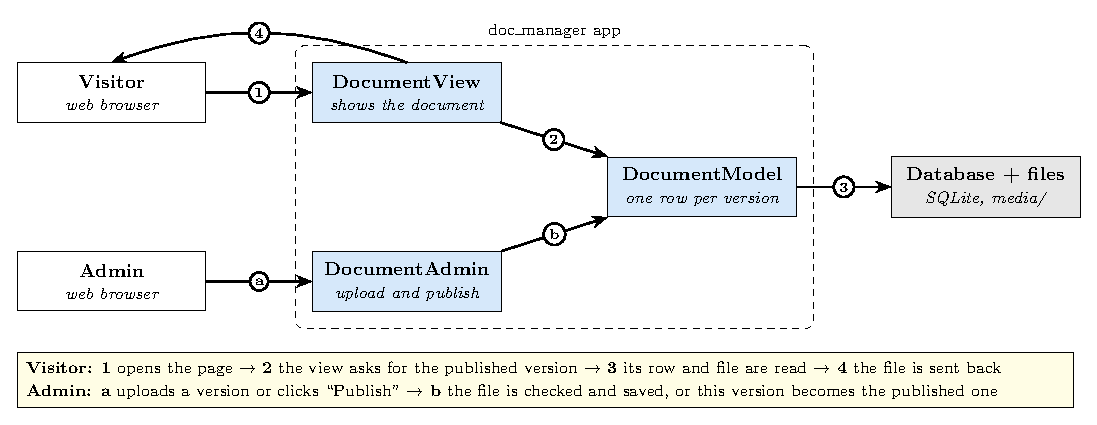
\includegraphics[width=0.78\linewidth]{../../Part1/pattern_architecture/architecture.pdf}
\end{frame}

\begin{frame}{The two patterns, in plain words}
\begin{columns}[T]
\column{0.5\linewidth}
\textbf{Template Method}\\[2pt]
A parent class owns a fixed \emph{recipe}.\\ A child class fills in one step.\\[6pt]
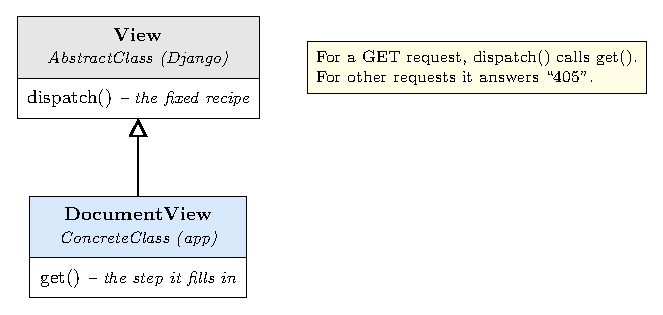
\includegraphics[width=0.8\linewidth]{../../Part1/pattern_architecture/TM1_published_document_page.pdf}
\column{0.5\linewidth}
\textbf{Strategy}\\[2pt]
An object keeps a \emph{replaceable helper}\\ and calls it the same way every time.\\[6pt]
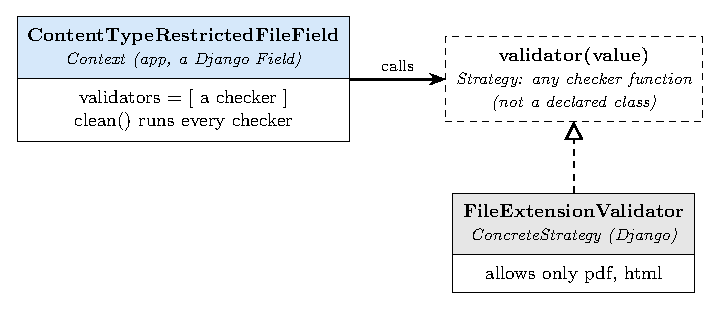
\includegraphics[width=0.95\linewidth]{../../Part1/pattern_architecture/S1_upload_file_checks.pdf}
\end{columns}
\end{frame}

\begin{frame}{Part 1 --- what we found: 2 types, 4 instances}
{\small\begin{tabular}{lll}\toprule
Instance & Pattern & Django part / app part\\\midrule
Published Document Page & Template Method & \code{View.dispatch} $\rightarrow$ \code{DocumentView.get}\\
Admin Read-only Fields & Template Method & \code{ModelAdmin} recipe $\rightarrow$ \code{get_readonly_fields}\\
Upload File Checks & Strategy & validators $\leftarrow$ \code{FileExtensionValidator}\\
Upload Widget Choice & Strategy & widget $\leftarrow$ \code{FileInput}\\\bottomrule
\end{tabular}}\par\vspace{10pt}
\begin{itemize}
\item Every instance is proven by a probe test that runs the real code (10/10).
\item 7 candidates rejected (e.g.\ Singleton, Decorator, Factory Method), 0 uncertain.
\end{itemize}
\end{frame}

\begin{frame}{Part 2 --- three changes, each with a small refactoring first}
\small\begin{tabular}{P{0.24\linewidth}P{0.27\linewidth}P{0.3\linewidth}l}\toprule
Change & Refactoring & Pattern effect & Tests\\\midrule
CH01 accept .txt files & Extract Constant: one \code{FILE_TYPES} table & 2 Strategy + 1 TM \emph{modified} & 11 $\rightarrow$ 19\\
CH02 open an older version & Extract Method \code{get_document()} & new TM ``Document Choice Step'' & 19 $\rightarrow$ 22\\
CH03 lock a published file & Rename Parameter & admin hook \emph{modified} & 22 $\rightarrow$ 25\\\bottomrule
\end{tabular}\\[10pt]
\begin{itemize}
\item New tests failed before each change and passed after; all logs are saved.
\item Instances: 4 $\rightarrow$ 4 $\rightarrow$ 5 $\rightarrow$ 5. LOC 138 $\rightarrow$ 158. Highest CC 5 $\rightarrow$ 4.
\end{itemize}
\end{frame}

\begin{frame}{Part 2 --- a new Template Method appeared (CH02)}
\centering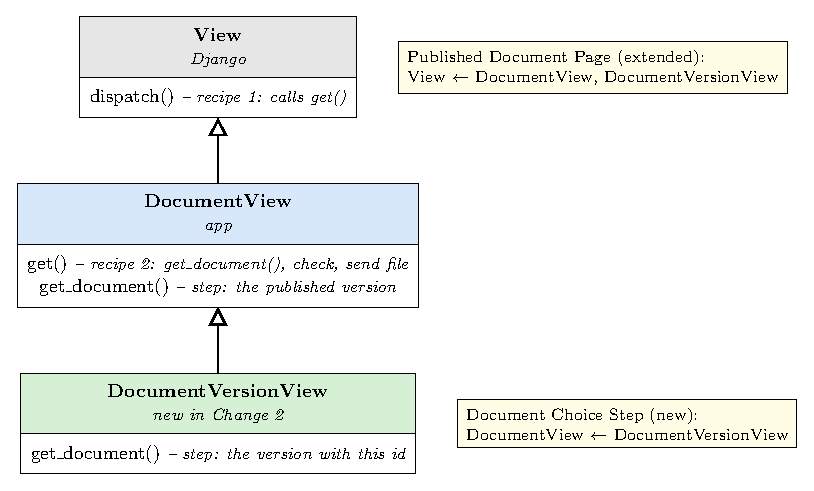
\includegraphics[width=0.62\linewidth]{../../Part2/diagrams/views_after_change2.pdf}\\[4pt]
\small The new class changes only \emph{one step}: which version to show (drafts stay hidden).
\end{frame}

\begin{frame}{Part 3 --- same problems in four languages}
\centering\begin{tabular}{lrrrrrr}\toprule
& \multicolumn{3}{c}{Template Method} & \multicolumn{3}{c}{Strategy}\\
Language & LOC & CC & ms & LOC & CC & ms\\\midrule
Python & 20 & 3 & 73.2 & 31 & 5 & 79.1\\
JavaScript & 28 & 3 & 80.2 & 40 & 5 & 78.7\\
Java & 30 & 3 & 201.8 & 51 & 5 & 224.7\\
C++ & 38 & 3 & 13.4 & 63 & 5 & 12.5\\\bottomrule
\end{tabular}\\[8pt]
\raggedright\begin{itemize}
\item All 8 programs pass the same shared cases (7/7 and 8/8).
\item Java and C++ catch a missing step at compile time; Python and JavaScript at run time.
\end{itemize}
\end{frame}

\begin{frame}{LLM use (Claude Opus 5.5) --- checked claim by claim}
\begin{tabular}{lcccl}\toprule
Part & Correct & Partial & Wrong & What we used\\\midrule
1 discovery & 11 & 1 & 2 & a missed instance (proven first)\\
2 evolution & 11 & 3 & 1 & warning: CH02 showed drafts $\rightarrow$ fixed\\
3 languages & 8 & 1 & 0 & generated code tested only (8/8 pass)\\\bottomrule
\end{tabular}\\[10pt]
\begin{itemize}
\item Prompts, inputs, raw outputs and our checks are saved for every run.
\end{itemize}
\end{frame}

\begin{frame}{Findings}
\begin{itemize}
\item Even a tiny Django app uses Template Method and Strategy: Django gives the fixed part, the app fills in the rest.
\item The patterns made each change small: one table entry, one step, one hook.
\item Refactoring first, with tests before and after, kept every change safe.
\item Bugs found: the page crashed for other file types and the \code{accept} hint was ignored (both fixed); the admin search crashes (documented).
\end{itemize}
\end{frame}

\end{document}
